\documentclass{beamer}

\graphicspath{ {../code/}}
\mode<presentation> {
%\usetheme{default}
%\usetheme{AnnArbor}
%\usetheme{Antibes}
%\usetheme{Bergen}
%\usetheme{Berkeley}
%\usetheme{Berlin}
%\usetheme{Boadilla}
%\usetheme{CambridgeUS}
%\usetheme{Copenhagen}
%\usetheme{Darmstadt}
%\usetheme{Dresden}
%\usetheme{Frankfurt}
%\usetheme{Goettingen}
%\usetheme{Hannover}
%\usetheme{Ilmenau}
%\usetheme{JuanLesPins}
%\usetheme{Luebeck}
%\usetheme{Madrid}
%\usetheme{Malmoe}
%\usetheme{Marburg}
%\usetheme{Montpellier}
%\usetheme{PaloAlto}
%\usetheme{Pittsburgh}
\usetheme{Rochester}
%\usetheme{Singapore}
%\usetheme{Szeged}
%\usetheme{Warsaw}

% As well as themes, the Beamer class has a number of color themes
% for any slide theme. Uncomment each of these in turn to see how it
% changes the colors of your current slide theme.

%\usecolortheme{albatross}
%\usecolortheme{beaver}
%\usecolortheme{beetle}
\usecolortheme{crane}
%\usecolortheme{dolphin}
%\usecolortheme{dove}
%\usecolortheme{fly}
%\usecolortheme{lily}
%\usecolortheme{orchid}
%\usecolortheme{rose}
%\usecolortheme{seagull}
%\usecolortheme{seahorse}
%\usecolortheme{whale}
%\usecolortheme{wolverine}
\useinnertheme{rectangles}

%\setbeamertemplate{headline}{}
\setbeamertemplate{footline} % To remove the footer line in all slides uncomment this line
%\setbeamertemplate{footline}[page number] % To replace the footer line in all slides with a simple slide count uncomment this line

\setbeamertemplate{navigation symbols}{} % To remove the navigation symbols from the bottom of all slides uncomment this line
}

\usepackage{graphicx} % Allows including images
\usepackage{booktabs} % Allows the use of \toprule, \midrule and \bottomrule in tables

%----------------------------------------------------------------------------------------
%   TITLE PAGE
%----------------------------------------------------------------------------------------

\title[Adaboost]{Voting Assemblies: Adaboost} % The short title appears at the bottom of every slide, the full title is only on the title page

\author{Jerry Bonnell, Gururaj Shriram, and Lloyd Beaufils} % Your name
\institute[ML] {ECE548 Group 7}
\date{\today} % Date, can be changed to a custom date

\begin{document}
{
\setbeamertemplate{headline}{}
\begin{frame}
\titlepage % Print the title page as the first slide
\end{frame}
}

%\begin{frame}
%\frametitle{Overview} % Table of contents slide, comment this block out to remove it
%\tableofcontents % Throughout your presentation, if you choose to use \section{} and \subsection{} commands, these will automatically be printed on this slide as an overview of your presentation
%\end{frame}

%----------------------------------------------------------------------------------------
%   PRESENTATION SLIDES
%----------------------------------------------------------------------------------------

%------------------------------------------------
\section{A bit of theory} % Sections can be created in order to organize your presentation into discrete blocks, all sections and subsections are automatically printed in the table of contents as an overview of the talk
%------------------------------------------------
\begin{frame}
\frametitle{Why bother \textbf{boosting}?}
\begin{itemize}
\item Data used for induction rarely captures all aspects of the class. % Variance error 
\item Individual classifiers suffer from \textbf{bias-related} error. % linear classifiers suffer from linearly separability 
\item How about using \textbf{many} classifiers? ``Collective wisdom''? 
\end{itemize}

\end{frame}
%------------------------------------------------
\begin{frame}
\frametitle{A bit of theory...}
\begin{block}{Adaboost}
``Examples are chosen from a probabilistic distribution that is gradually modified in a way that makes the whole ``assembly'' focus on those aspects that appear to be difficult.''\\
- Miroslav Kubat, \textit{An Introduction to Machine Learning}
\end{block}
\begin{itemize}
\item Improvement over \textbf{bagging} and \textbf{Schapire's boosting}. 
\begin{itemize}
\item Reduce randomness and the need for great many examples.
\end{itemize}
\item Classifiers should build upon the weaknesses of others. 
\end{itemize}

\end{frame}
%------------------------------------------------
\begin{frame}
\frametitle{A Practical Approach}
\begin{itemize}
\item Selecting examples for T\textsubscript{i} is done \textbf{probabilistically}. 
\item For T\textsubscript{1}: each example has $p = 1 / m$
\begin{itemize}
\item "Wheel of Fortune" 
\end{itemize}
\item For each following \textit{T}\textsubscript{i}: 
\begin{itemize}
\item Calculate $\varepsilon\textsubscript{i} = \sum_{j=1}^{m} p\textsubscript{i}(\textbf{x}\textsubscript{j}) * e\textsubscript{i}(\textbf{x}\textsubscript{j})$
\item Calculate $\beta\textsubscript{i} = \varepsilon\textsubscript{i} / (1 - \varepsilon\textsubscript{i}) $
\end{itemize}
\item Scale \textbf{correctly} classified examples by $p\textsubscript{i+1}(\textbf{x}\textsubscript{j}) = p\textsubscript{i}(\textbf{x}\textsubscript{j}) * \beta\textsubscript{i}$
\begin{itemize}
\item Less chance of being selected. 
\end{itemize}
\item Normalize to ensure the new distribution sums to 1.  
\item From each ``custom'' T\textsubscript{i}, a C\textsubscript{i} is induced.
\end{itemize}
\end{frame}
%------------------------------------------------
\begin{frame}
\frametitle{Weighted Majority Voting}
\begin{itemize}
\item Each classifier's vote has a weight.
\item Higher classifier performance = votes worth more = higher weight
\item Sum these weights for W\textsubscript{pos} and W\textsubscript{neg} to see which has higher support. 
\item How to obtain these weights? Use \textbf{perceptron learning}. 
\begin{itemize}
\item Present the assembly one example at a time from the training set.
\item Upon misclassification, use classical weight-updating formula (Chapter 4)
\end{itemize}
\end{itemize}

\end{frame}
%------------------------------------------------
\begin{frame}
\frametitle{Hypothesis}
\begin{itemize}
\item Training and testing error rate should \textbf{decrease} when more classifiers added. 
\begin{itemize}
\item We would like to see weak learners approximate the accuracy of a strong learner.
\end{itemize}
\item Error rate should \textbf{converge} after some large number of classifiers.
\item Computational costs $\rightarrow$ reap benefits of using small training subsets. 
\end{itemize}
\end{frame}
%------------------------------------------------
\begin{frame}
\Huge{\centerline{Does experience agree?}}
\end{frame}
%------------------------------------------------
\begin{frame}
\frametitle{Implementation}
\begin{itemize}
\item Weak learner: \textbf{Perceptron} (ours, in Python)
\item Strong learner: \textbf{Decision Tree} (Scikit)
\item Learning rate $\eta = 0.05$ and $\eta\textsubscript{weights} = 0.0001$ 
\item Threshold $\theta = 0.05$ and $\theta\textsubscript{weights} = 0.10$
\item Each training subset T\textsubscript{i} will hold 20\% of the training set.
\item Training set 65\% / Testing set 35\%
\end{itemize}
\end{frame}
%------------------------------------------------
\begin{frame}
\frametitle{Experiment}
\begin{itemize}
\item Begin with one learner. Add groups of two till 50 reached. 
\item Average this process for 5 times.  
\item Measure \textbf{\# classifiers} vs. \textbf{error rate} 
\end{itemize}
\end{frame}
%------------------------------------------------
\begin{frame}
\frametitle{Domains}
\begin{block}{UCI Repository}
\begin{enumerate}
\item \textbf{Musk} {\footnotesize{(168 attributes, 476 instances, 47 pos / 45 neg)}}
\item \textbf{Ionosphere} {\footnotesize{(34 attributes, 351 instances, 225 pos / 126 neg)}}
\item \textbf{insert} {\footnotesize{(xx attributes, xx instances, xx pos / xx neg)}}
\end{enumerate}
\end{block}
\begin{itemize}
\item Exclusively \textbf{binary} classification tasks. 
\end{itemize}
\end{frame}
%------------------------------------------------
\begin{frame}
\frametitle{Musk}
Insert graph here 
\end{frame}
%------------------------------------------------
\begin{frame}
\frametitle{Musk}
Insert another graph here 
\end{frame}
%------------------------------------------------
\begin{frame}
\frametitle{Musk Observations}
Insert another graph here 
\end{frame}
%-------------------------------------------------
\begin{frame}
\frametitle{Ionosphere}
\begin{center}
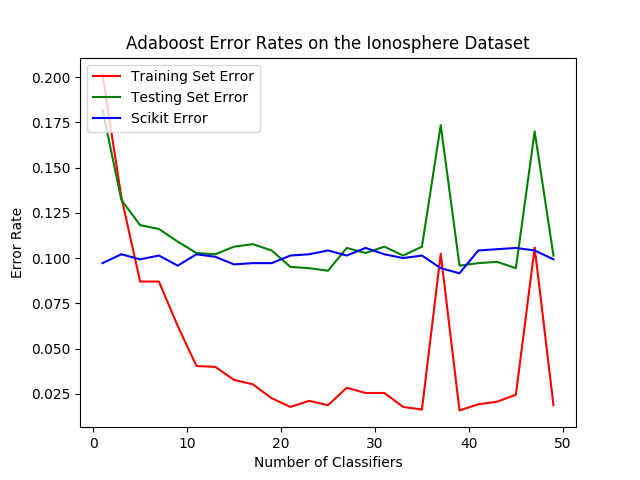
\includegraphics[width=0.8\linewidth]{Ionosphere.png}
\end{center}
\end{frame}
%------------------------------------------------
\begin{frame}
\frametitle{Ionosphere}
\begin{center}
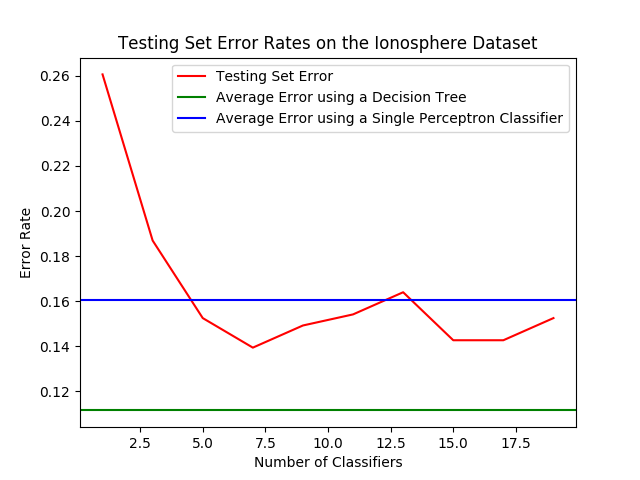
\includegraphics[width=0.8\linewidth]{Ionosphere_different_classifiers.png}
\end{center}
\end{frame}
%------------------------------------------------
\begin{frame}
\frametitle{Ionosphere Observations}
\begin{itemize}
\item observation 
\end{itemize}
\end{frame}
%-------------------------------------------------
\begin{frame}
\frametitle{Insert}
\begin{center}
%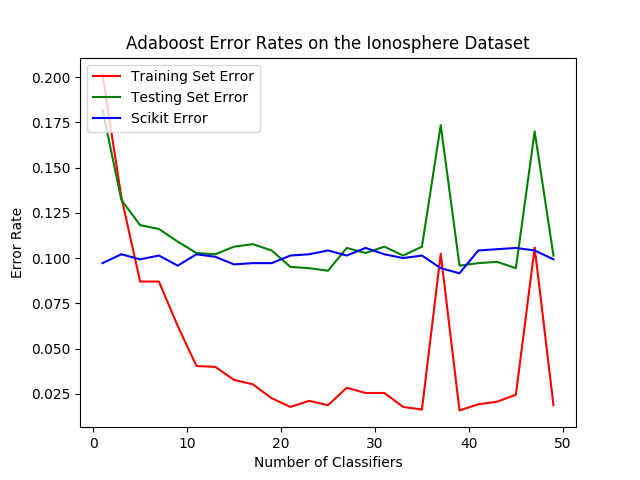
\includegraphics[width=0.8\linewidth]{Ionosphere.png}
graph here
\end{center}
\end{frame}
%------------------------------------------------
\begin{frame}
\frametitle{Insert}
\begin{center}
%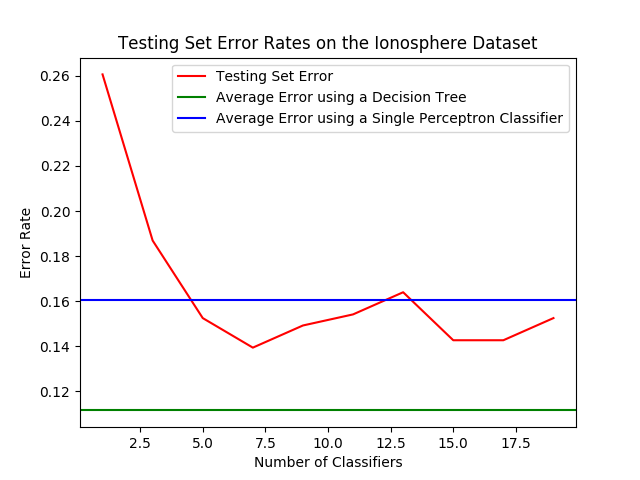
\includegraphics[width=0.8\linewidth]{Ionosphere_different_classifiers.png}
graph here 
\end{center}
\end{frame}
%------------------------------------------------
\begin{frame}
\frametitle{Insert Observations}
\begin{itemize}
\item observation 
\end{itemize}
\end{frame}
%------------------------------------------------
\begin{frame}
\frametitle{Conclusions}
\begin{itemize}
\item concluding remarks 
\end{itemize}
\end{frame}
%------------------------------------------------
\begin{frame}
\Huge{\centerline{Questions?}}
\end{frame}
%-----------------------------------------------

% \begin{frame}
% \frametitle{Multiple Columns}
% \begin{columns}[c] % The "c" option specifies centered vertical alignment while the "t" option is used for top vertical alignment

% \column{.45\textwidth} % Left column and width
% \textbf{Heading}
% \begin{enumerate}
% \item Statement
% \item Explanation
% \item Example
% \end{enumerate}

% \column{.5\textwidth} % Right column and width
% Lorem ipsum dolor sit amet, consectetur adipiscing elit. Integer lectus nisl, ultricies in feugiat rutrum, porttitor sit amet augue. Aliquam ut tortor mauris. Sed volutpat ante purus, quis accumsan dolor.

% \end{columns}
% \end{frame}

% %------------------------------------------------
% \section{Implementation}
% %------------------------------------------------

% \begin{frame}
% \frametitle{Table}
% \begin{table}
% \begin{tabular}{l l l}
% \toprule
% \textbf{Treatments} & \textbf{Response 1} & \textbf{Response 2}\\
% \midrule
% Treatment 1 & 0.0003262 & 0.562 \\
% Treatment 2 & 0.0015681 & 0.910 \\
% Treatment 3 & 0.0009271 & 0.296 \\
% \bottomrule
% \end{tabular}
% \caption{Table caption}
% \end{table}
% \end{frame}

% %------------------------------------------------

% \begin{frame}
% \frametitle{Figure}
% Uncomment the code on this slide to include your own image from the same directory as the template .TeX file.
% %\begin{figure}
% %\includegraphics[width=0.8\linewidth]{test}
% %\end{figure}
% \end{frame}

%------------------------------------------------


\end{document}
              